\documentclass{article} % For LaTeX2e
\usepackage{nips14submit_e,times}
\usepackage{hyperref}
\usepackage{url}
\usepackage[utf8]{inputenc}
\usepackage{amsmath}
\usepackage[numbers,sort]{natbib}
\usepackage{graphicx}
\usepackage[export]{adjustbox}
\usepackage{footmisc}
\DeclareGraphicsExtensions{.pdf,.png,.jpg,.eps}

%\documentstyle[nips14submit_09,times,art10]{article} % For LaTeX 2.09         



\author{
Gabriel C-Parent\\
Département d’informatique et recherche opérationnelle\\
Université de Montréal\\
\texttt{gabriel.c-parent@umontreal.ca} \\
\And
Dora Fugère \\
Département de mathématiques et de statistique \\
Université de Montréal\\
\texttt{dora.fugere@umontreal.ca} \\
}


\newcommand{\fix}{\marginpar{FIX}}
\newcommand{\new}{\marginpar{NEW}}

\nipsfinalcopy % Uncomment for camera-ready version

\begin{document}


\title{Fool me once, shame on - shame on you. \newline
       Fool me - can't get fooled again.}
      
\maketitle

\begin{abstract}
% still needs much work
Adversarial examples generation from input space in neural network
has shown that these powerful constructs can be manipulated into misclassifying previously well classified examples by adding an imperceptible
amount of distortion.

Using this methodology, we investigate the relative robustness to distortion of a simple linear SVM with
hinge loss and some regularization schemes.
\end{abstract}


\section{Introduction}

% new problems vs progress
Recently, neural networks have been brought under questioning. The smoothness
assumption, the idea that imperceptible distortion of input shouldn't change
the output was shown not to hold \citep{szegedy_intriguing_2013}. This is a
remarkable finding since smoothness was assumed to be a necessary property of the
learning process.
This comes in stark constrast with feats such as automatic image description
\citep{vinyals_show_2014} and large-scale multi-character text recognition
\citep{goodfellow_multi-digit_2013} to name but a few.

% comprehensibility is important
As for most real-world problems, there are many desirable and often conflicting
goals when using machine learning. Amongst them speed, accuracy and simplicity
are easy to justify. We'll focus on comprehensibility, because that justifies
us using a simpler model.
We interpret simplicity as ``given two models with the same generalization error, the more
comprehensible one should be preferred" \citep{domingos_role_1999}.
This obviously is dependent on multiple other factors (e.g. speed and accuracy)
but it does sound like the \textit{keep it simple stupid} rule of thumb.
Furthermore, as stated in \citep{hand_classifier_2006}, empirical comparison of
performance is very context-dependent and can be infludenced by treatments such 
as the preprocessing steps, training parameters and model hyperparameters.

% experiments executed
Inspired by the methodology to induce misclassification, we wondered
if a similar optimization procedure could be applied to generate adversarial
examples in a simpler classifier. For this purpose, we used a support vector machine (SVM) with hinge loss and $L_1$, $L_2$ and $elasticnet$-regularization. The only other contender would have been Naive Bayes,
but we happen to like sklearn's implementation of the linear SVM \footnote{we wouldn't
risk reinventing the square wheel} \citep{pedregosa_scikit-learn:_2011}.
We report the robustness of our optimization procedure, the results on classifiers
trained with different loss and regularization parameters and we then feed the 
generated adversarial examples to a neural network to see if some underlying
feature of the image was captured.


%%%%%%%%%%%%%%%%%%%%%%%%%%%%%%%%%%%%%%%%%%%%%%%%%%%%%%%%%%%%%%%%%%%%%%%%%%%%%%%
%%%%%%%%%%%%%%%%%%%%%%%%%%%  FRAMEWORK %%%%%%%%%%%%%%%%%%%%%%%%%%%%%

\section{Framework}


\subsection{Dataset}

The experiments were performed on the MNIST dataset \citep{lecun_mnist_1998}.

Let \begin{math} X=\{0, 255\}^{784} \end{math}, the input domain.
This is the set of $28\times28$ 8-bit grayscale image.

Let \begin{math} Y = \{0, 9\} \end{math}, the output domain.
This is the set of valid classes for an MNIST digit.


\subsection{Preprocessing}

The MNIST dataset was deskewed and brought back to 8-bit data. This improved the performance of the classifier.


\subsection{Optimization goal}

Let \begin{math} f:X \rightarrow  Y \end{math} a classifier mapping $x_i \in
X$ to $y_i \in Y$.

We aim to solve the following optimization

\begin{equation}
\label{eq:optimization}
\begin{aligned}
& {\text{minimize}}
&   \lVert{r} \rVert^2\\
& \text{subject to} \\
& & x_i + r \in X \\
& & f(x_i) \neq f(x_i + r)
\end{aligned}
\end{equation}

This is quite similar to \citep{szegedy_intriguing_2013} but the newly
generated images remain 8-bit to stay in the input domain of the MNIST dataset.
Sadly, this also makes it a discrete optimization problem.


\subsection{Optimization goal for the linear SVM}

We denote $\widehat{y_i}$ the correct class for $x_i$. Given a correctly
classified $x_i$, the objective is to find a vector of distortion $r$ such that $f(x_i + r) \neq  \widehat{y_i}$.

In a two-class setting, the classifier classifies the input based on the following decision function.

\begin{equation}
\label{eq:decision_function}
  y_i = argmax (x_i \cdot W^T + b)
\end{equation}

Suppose that $\widehat{y_i} = 1$, the correct class is 1.The difference between the class weights (coefficients) of the classifier is $W_d$.
It is obtained by subtracting the coefficients of the goal class (2 in 
this case) by $\widehat{y_i}$'s.

\begin{equation}
\label{eq:difference}
  W_d = W_2 - W_1
\end{equation}

The distance between the values of the two classes is $d$.
\begin{equation}
\label{eq:gap}
  d = x_i \cdot W_d^T
\end{equation}


To cause misclassification, $r$ must respect the following constraint:
\begin{equation}
\label{eq:noise_threshold}
  r \cdot W_d^T > d
\end{equation}

What we need is to find the smallest $ \lVert{r} \rVert^2$ that will cause
misclassification. 

Note that when there are more than two classes, we just
apply the procedure to all other classes $y \neq \widehat{y_i}$ and choose the one with minimal squared euclidean norm.

The distorted set of images is generated by applying the following function over
the input images.
\begin{equation}
	\label{robustness}
	distorted(x_i) = min(\{\lVert{r_{y}} \rVert^2 \mid y \neq \widehat{y_i}\})
\end{equation}
where $\widehat{y_i}$ is the true and predicted class of the $i$th image and $\lVert{r_{y}} \rVert^2$ the smallest squared euclidean norm needed for the classifier to classify it as $y$.


\subsection{Knapsack problem and the greedy approach}

The problem is similar to the bounded multiple-class binary Knapsack problem
\citep{vanderbeck_extending_2002}, with the difference that we are searching
for the smallest knapsack holding a value superior to $d$ (equation
\ref{eq:gap}).

The exact algorithm would be too costly for our purpose so we chose to use a
greedy heuristic inspired by Dantzig's \citep{dantzig_discrete-variable_1957}.

The procedure is described in more details in section \ref{greedy:proof}.


%%%%%%%%%%%%%%%%%%%%%%%%%%%%%%%%%%%%%%%%%%%%%%%%%%%%%%%%%%%%%%%%%%%%%%%%%%%%%%%
%%%%%%%%%%%%%%%%%%%%%%%%%%%  EXPERIMENTAL RESULTS %%%%%%%%%%%%%%%%%%%%%%%%%%%%%

\section{Experimental results}



%==============================================================================

\subsection{Precision of optimization procedure}

Although the bounds on the optimization procedure could be arbitrary big, it
is usually small for this problem, because $d$ is usually quite big relative
to the size of weight increments. This means tight bounds on the possible
true value of the squared euclidean norm.

\begin{figure}[h!]
\begin{center}
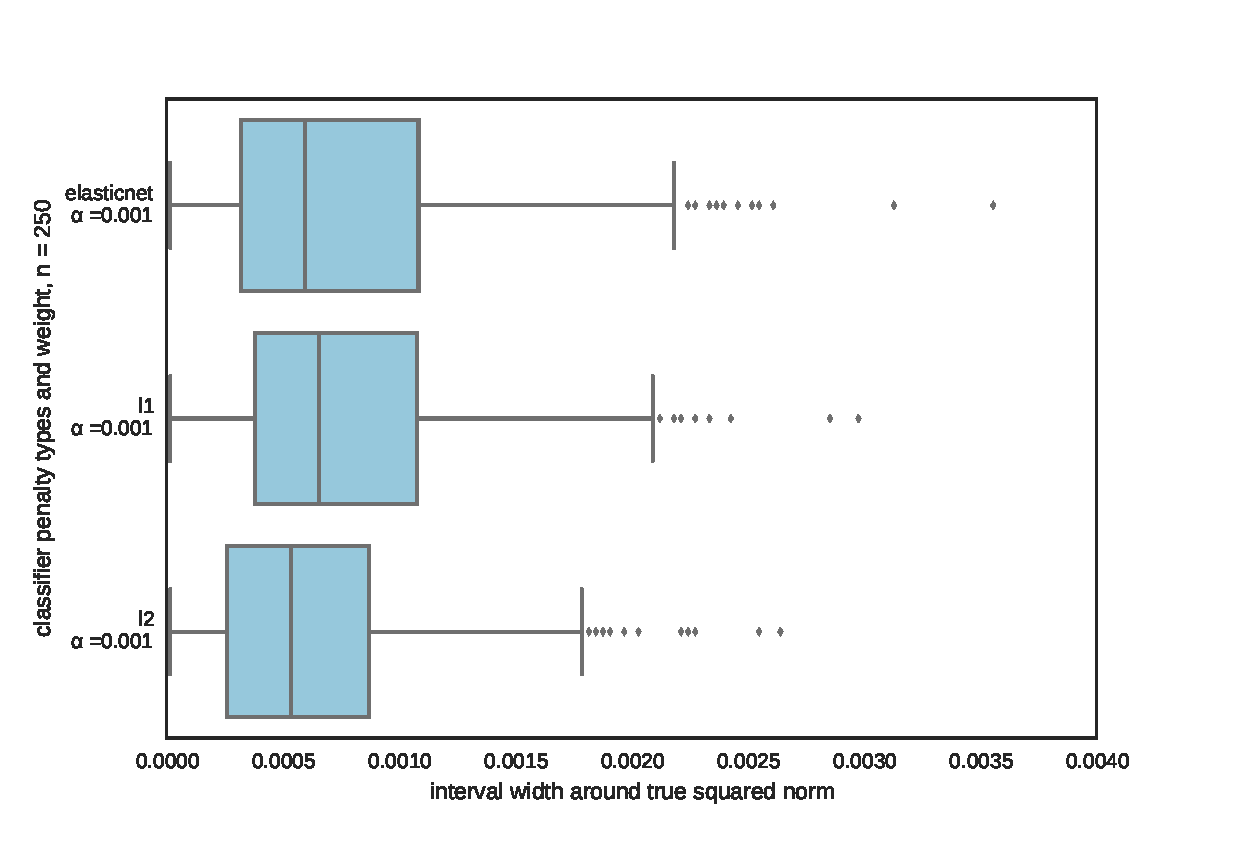
\includegraphics[scale=0.65]{figs/experiment_1}
\label{res:exp1}
\caption{\small Size of the interval on the true value of the minimal squared norm for various
                classifier on the MNIST dataset. The bound is shown to be very tight, especially considering the usual size of $d$.}
\end{center}
\end{figure}

Since the bound on the true optimal value is always very tight, the use of
the greedy optimization procedure is reasonable.

%==============================================================================

\subsection{Regularization schemes}

We wanted to observe the effects of different regularization methods and parameters on the examples. To do so, we started with
a pilot run, to assess the potential of the various configurations.

The most promising regularization penalty was the $L_2$-norm (ridge
regression) penalty and its results are shown here. 
The complete results can be viewed in figure \ref{exp:sup_2} of the supplementary material.

\begin{figure}[h!]
 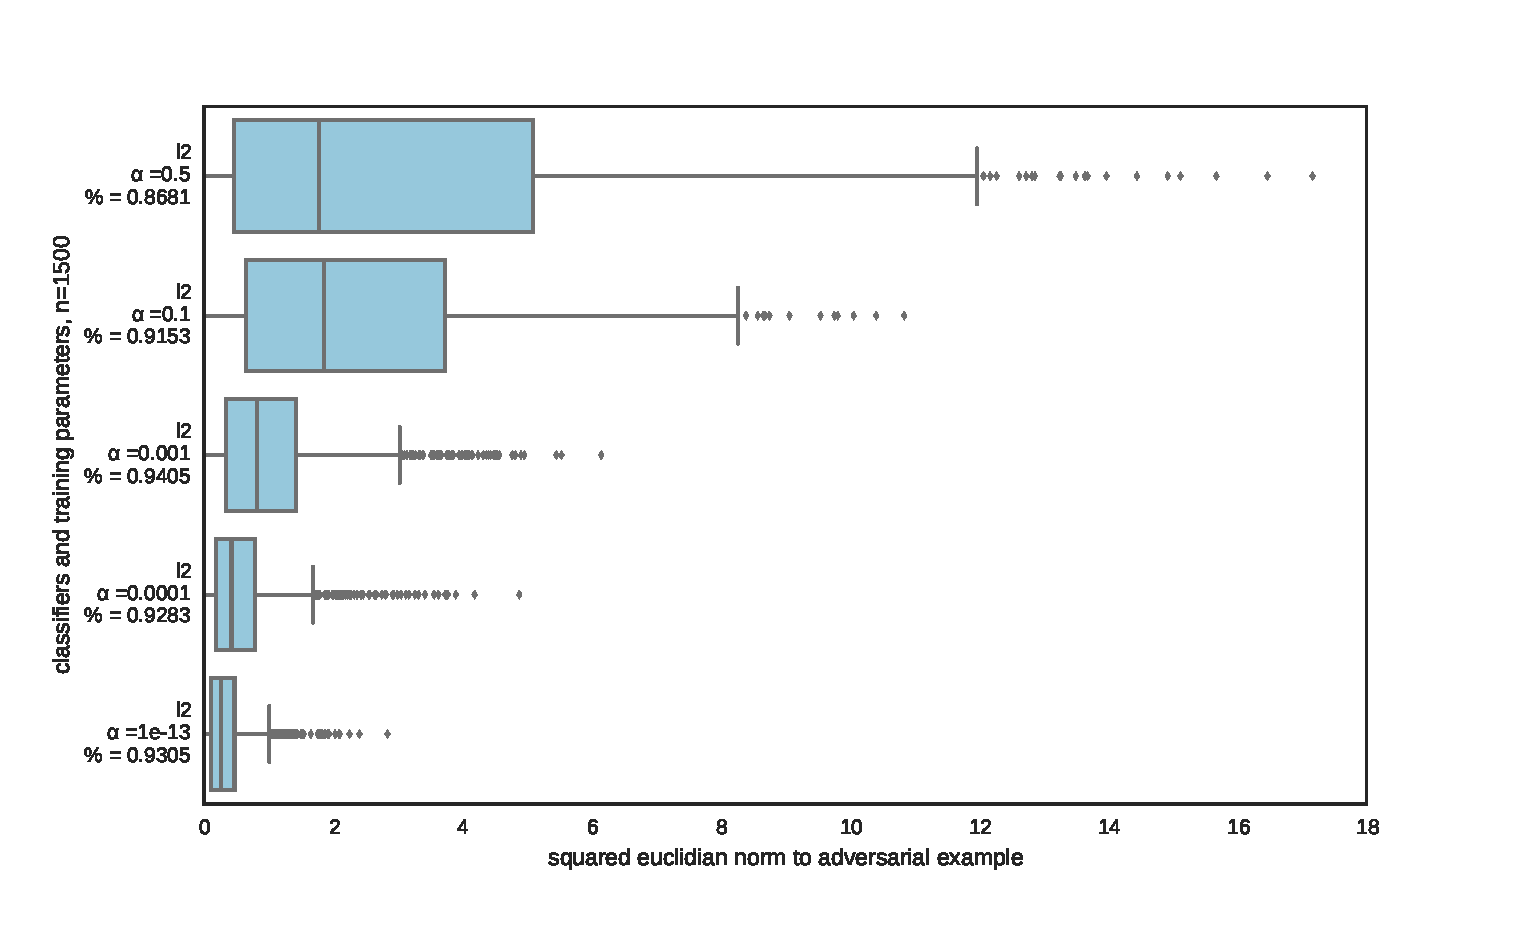
\includegraphics[scale=0.5]{figs/experiment_2_l2}
 \label{res:exp2}
 \caption{\small Improvement of robustness with regularization for the $L_2$-regularized SVM with hinge loss. The improvement in squared euclidean norm is very apparent as the value of $\alpha$ goes up.}
\end{figure}


%==============================================================================


\section{Discussion}

As expected, higher regularization penalty yields better robustness to distortion. This comes with the cost of decreasing generalization accuracy when the strength is too high. This got the $L^1$-regularized classifiers to fail early, as their accuracy decreased below the fixed threshold we chose (85\% of generalization accuracy) very quickly, without much impact on robustness. This is show in figure \ref{exp:sup_2}.

From the observations in figure \ref{res:exp2}, we chose the $L^2$-regularized classifier with regularization term 0.5 for further experiments because it had the highest robustness to distortion.

We went on to explore a few aspects of the distortion. The first interesting property for our classifier was the non-uniformity of distribution of adversarial examples as shown in figure \ref{exp_sup3}. It is quite interesting to see the relation between original and closest class by distortion.

It is furthermore interesting to observe that some input classes are more robust (especially the ones, but it makes sense since the MNIST dataset was preprocessed to straighten them). The distribution of squared euclidean norms for adversarial examples is presented in figure \ref{exp:sup_4}.
To further the point, selected examples of digits and
their adversarial class counterpart we selected and are
shown in figure \ref{exp:sup_5}. The smallest, median and largest required distortions were selected to give an idea of the range of distortion and the visual impact it has on the input images when using the optimization procedure. It must be remembered that the distortion can consist of adding or removing intensity by 1 bit increments and the resulting adversarial
examples are valid 8-bit grayscale images.

Some additional work was done on cross-training-set generalization between two classifiers ($L^2$-regularized, $\alpha=0.5$, same as before). The 60000 MNIST dataset was split in two disjoint sets, as in \citep{szegedy_intriguing_2013}.
%The results are shown in figure \ref{exp:sup_6}




\subsubsection*{Acknowledgments}
We would like to thank Red Bull, it gives you wings\footnote{No it doesn't. Don't sue them again.}.


\bibliographystyle{plain}


\bibliography{project}


%%%%%%%%%% supplemental materials %%%%%%%%%%
\newpage


\begin{center}
\textbf{\large Supplementary Materials}
\end{center}

\subsection{greedy optimization heuristic, the nitty–gritty details}
\label{greedy:proof}

Let $S = (o_1 , ..., o_n)$ be objects sorted in decreasing unit-value order i.e. value($o_i$)/volume($o_i$) $\geq$  value($o_{i+1}$)/volume($o_{i+1}$).

If $K$ is a choice of the first $k$ items of $S$ and $V=volume(K)$, then a knapsack of size $V$ would be optimal for the objects of $S$. This is intuitive since no other choice would have a better value/cost ratio. This is the crux of the matter for our optimization procedure.


Let $(K_1, V_1)$ and $(K_2, V_2)$, the volumes and values of two optimal knapsacks. We know that if $K_1 < K_2$ then $V_1 \leq V_2$, for we could choose the elements of $K_1$ to get an equal value or find better. This also means that given $V_1 < V_3 < V_2$ then $K_1 < K_3 < K_2$. This allows us to find bounds on $K_3$ if we know $(K_1, V_1)$ and $(K_2, V_2)$, as it must be squeezed between the two.

%It is possible to encode the cost of adding a bit of distortion to a pixel in the form of a volume and the gradient of improvement (eq. \ref{eq:difference}) can be encoded as the volume. This
%is acceptable because each time distortion is added, we add a new object to $S$ and its value/volume is guaranteed to be lower than the latest optimal (we have squared euclidean norm) so it would not have been chosen before.
%
%For example, given vector of distortion $r$ = [0, 3], the costs of
%adding 1 unit of distortion for each position of $r$ is [1, 7]. For the values,
%we use the absolute value of vector $W_d$. If $W_d$ = [-5, 10], the 
%$\frac {value} {volume}$ ratios would be [5, $\frac{10}{7}$]. The best choice
%to improve the value 
%
%We iteratively choose the elements with the best until
%the critical value is $d$ is passed.
%
%At iteration $n$, the choices made are optimal of the knapsack of size
%$K_n = \sum\limits_{i=1}^n w_i$. This is the case because every object in the
%knapsack was chosen with maximum $\frac{value} {volume}$ ratio and the knapsack
%is filled perfectly.
%
%
%
%For our purpose, this means that the true value of the norm
%$\lVert{r} \rVert^2 \in [K_{n-1}, K_n]$ if the algorithm finishes at iteration
%$n$. This boundary can be very small or very big, depending on the size of the
%weight increments. We measured the boundary size to show that in this problem,
%we have very little incertitude.

\newpage
\subsection{regularization methods and robustness}

\begin{figure}[h!]

\begin{center}
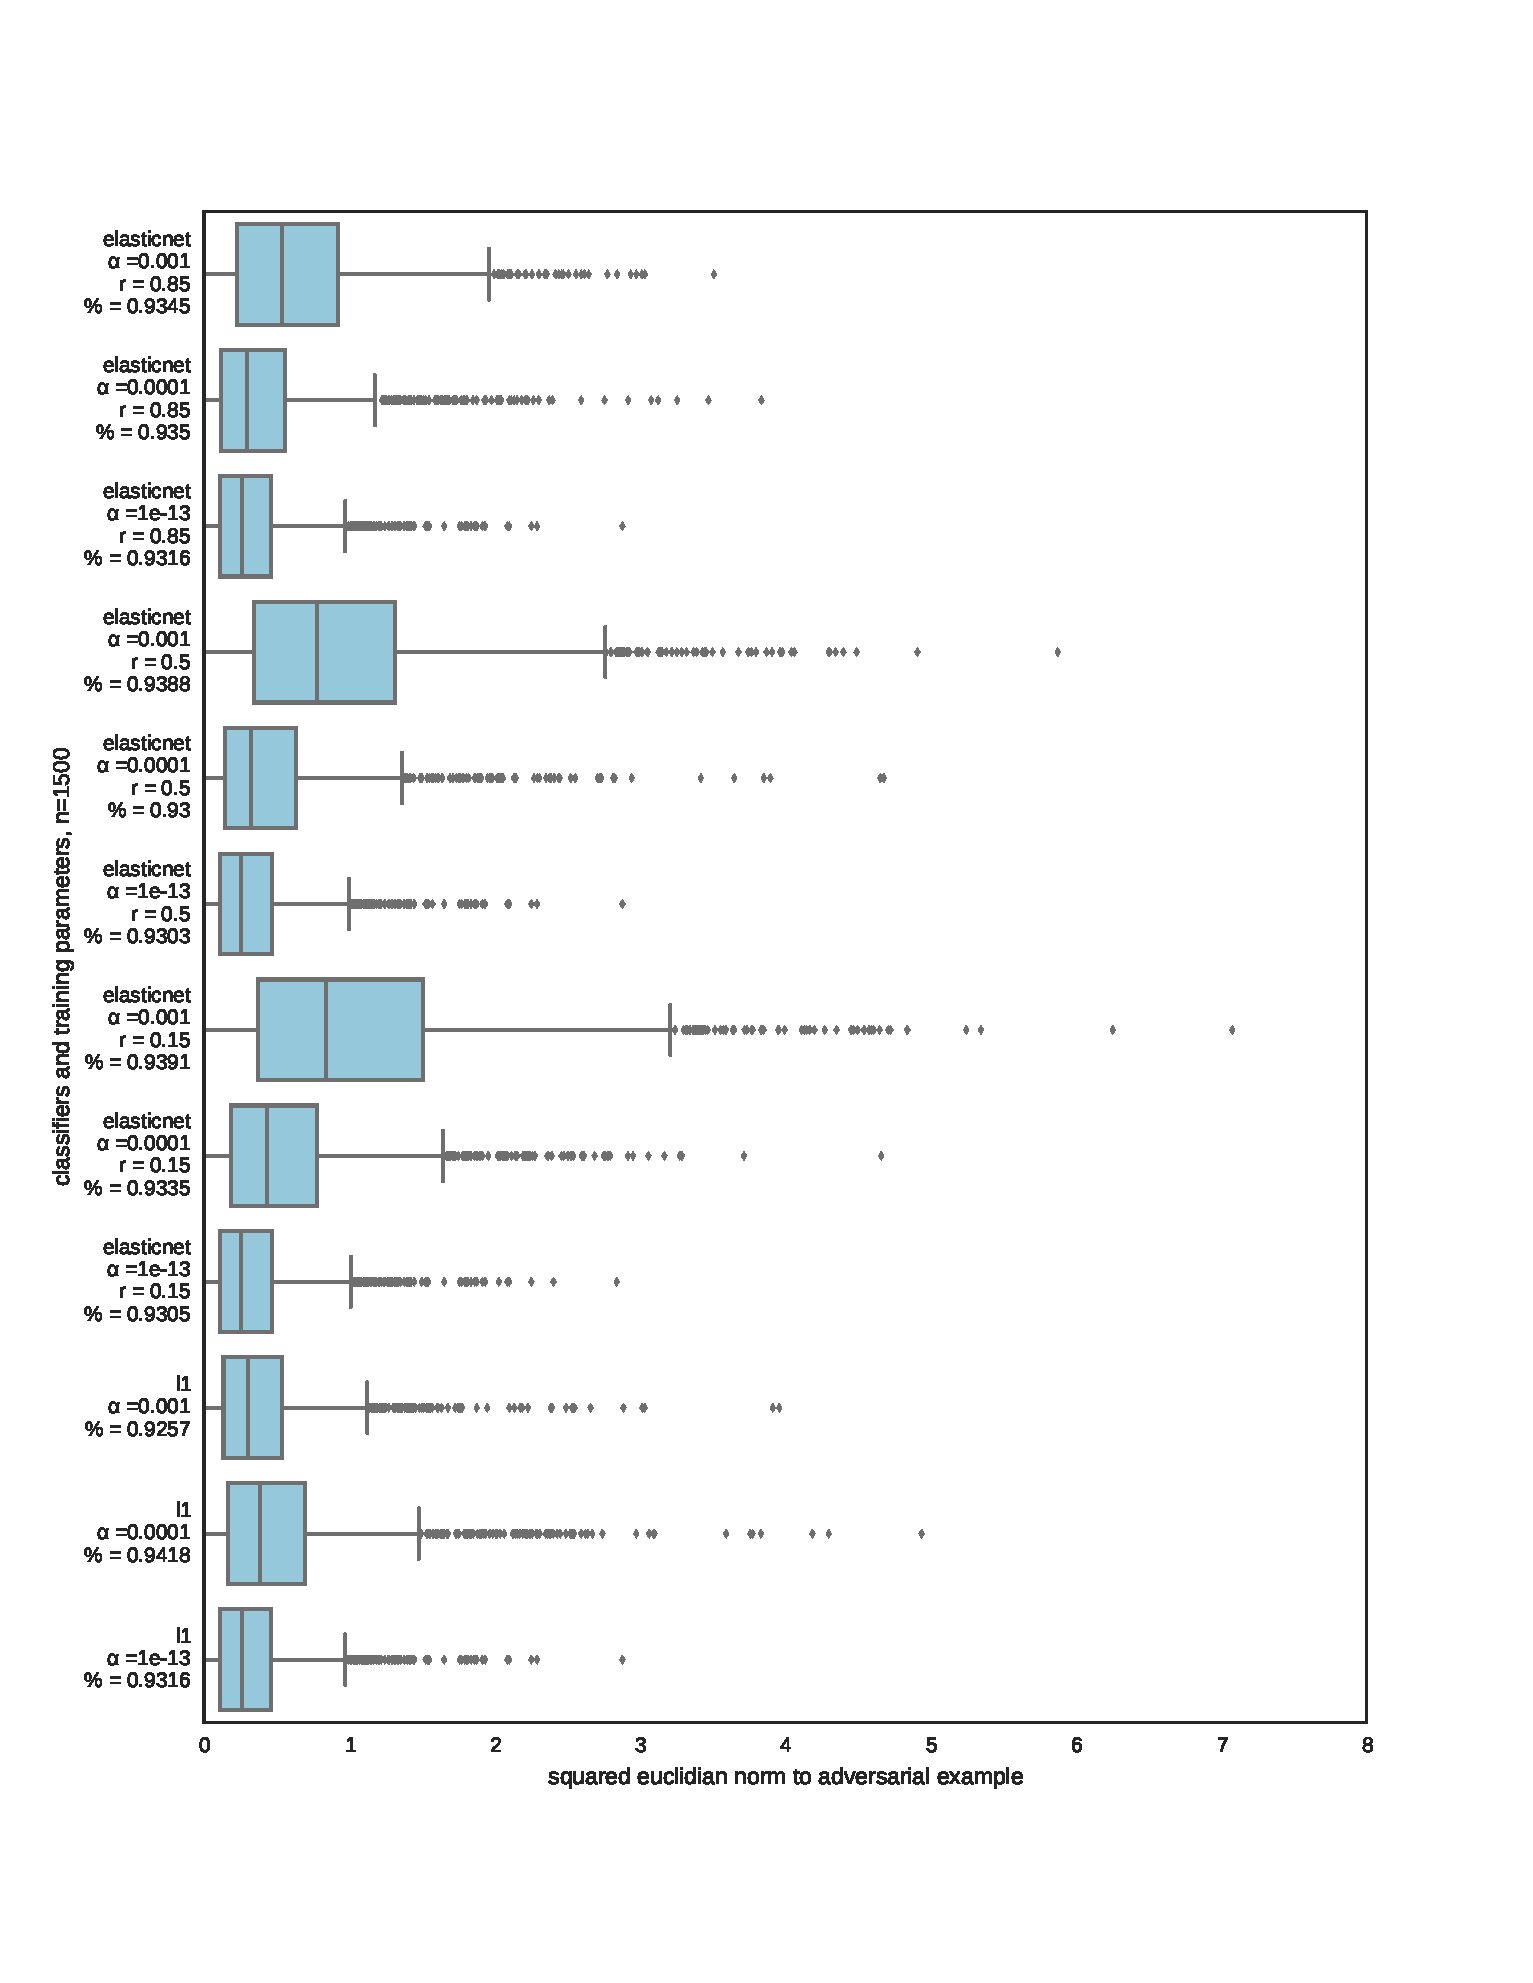
\includegraphics[scale=0.5]{figs/sup_1}
\label{exp:sup_2}
\end{center}
\caption{\small Less successful classifiers. Squared euclidian norm is relatively small in comparison to $L_2$ penalty. We see improvement as the coefficient of the penalty grows bigger.}
\end{figure}


\null
\vfill
\newpage


\subsection{comparison of robustness of two classifiers}

\begin{figure}[h!]
\begin{center}
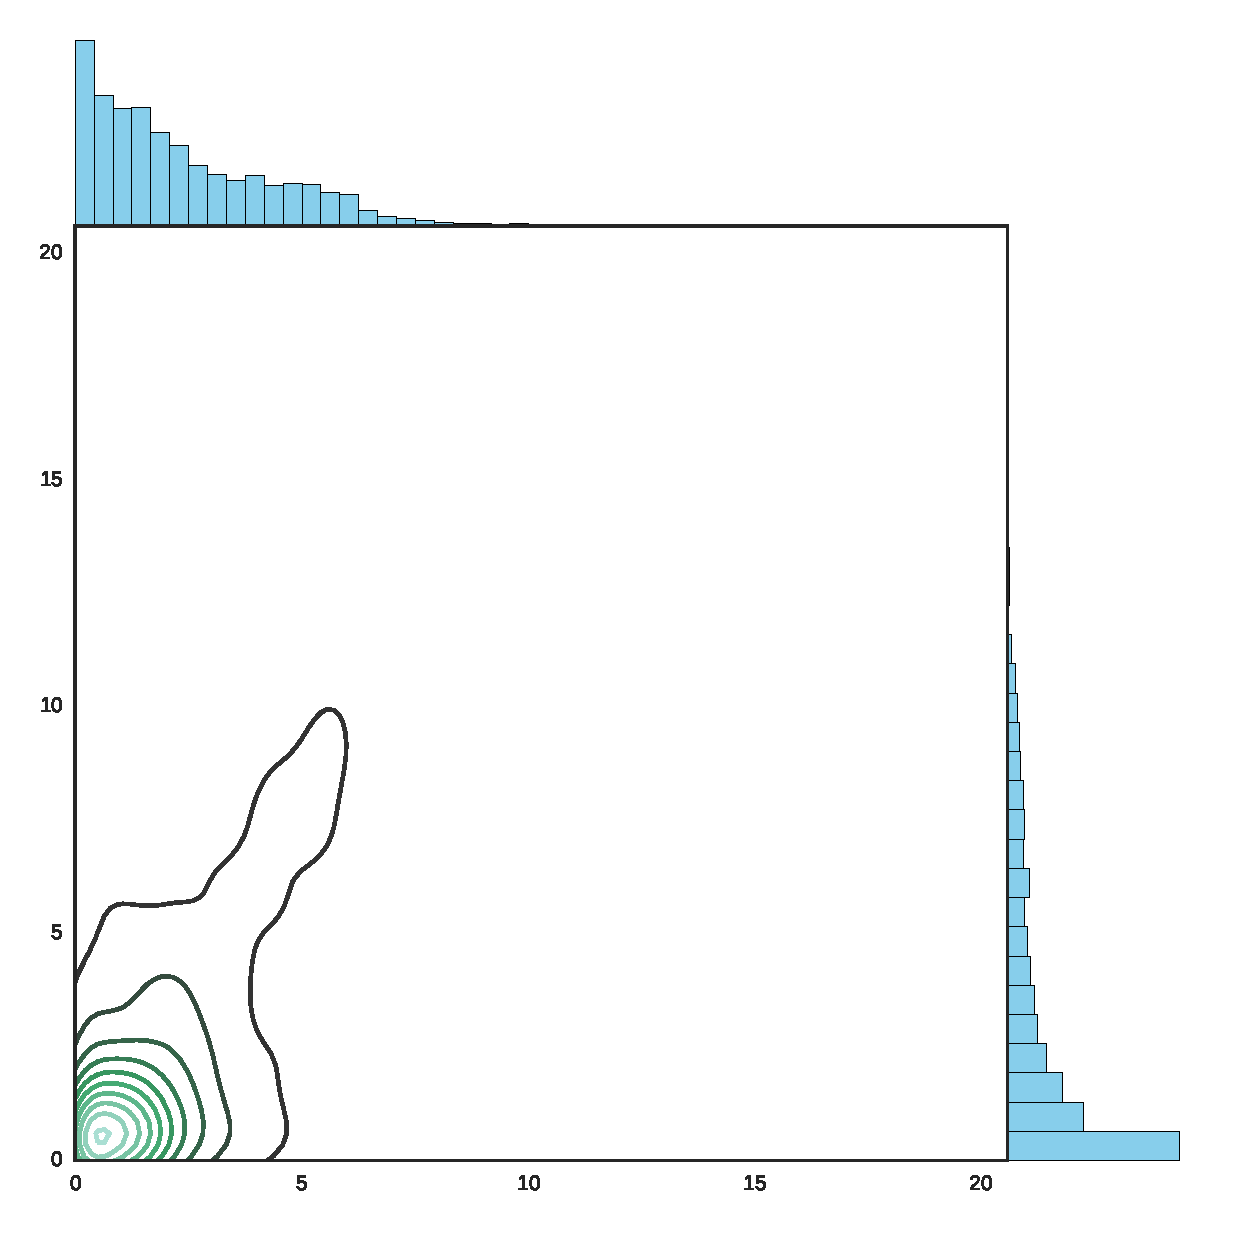
\includegraphics[scale=0.6]{figs/sup_2}
\label{exp:sup_2}
\caption{\small Comparison of the distribution of the squared norm for distorted images. The last same two classifiers as in figure \ref{res:exp2} were compared.
The classifier with bigger $\alpha$ is yielding bigger squared euclidean norm (the angle of the density allows us to tell). This means that the classifier is more robust to distortion.}
\end{center}
\end{figure}

\null
\vfill
\raggedbottom
\pagebreak
\newpage

\subsection{example of transitions}

\begin{figure}[h!]
\begin{center}
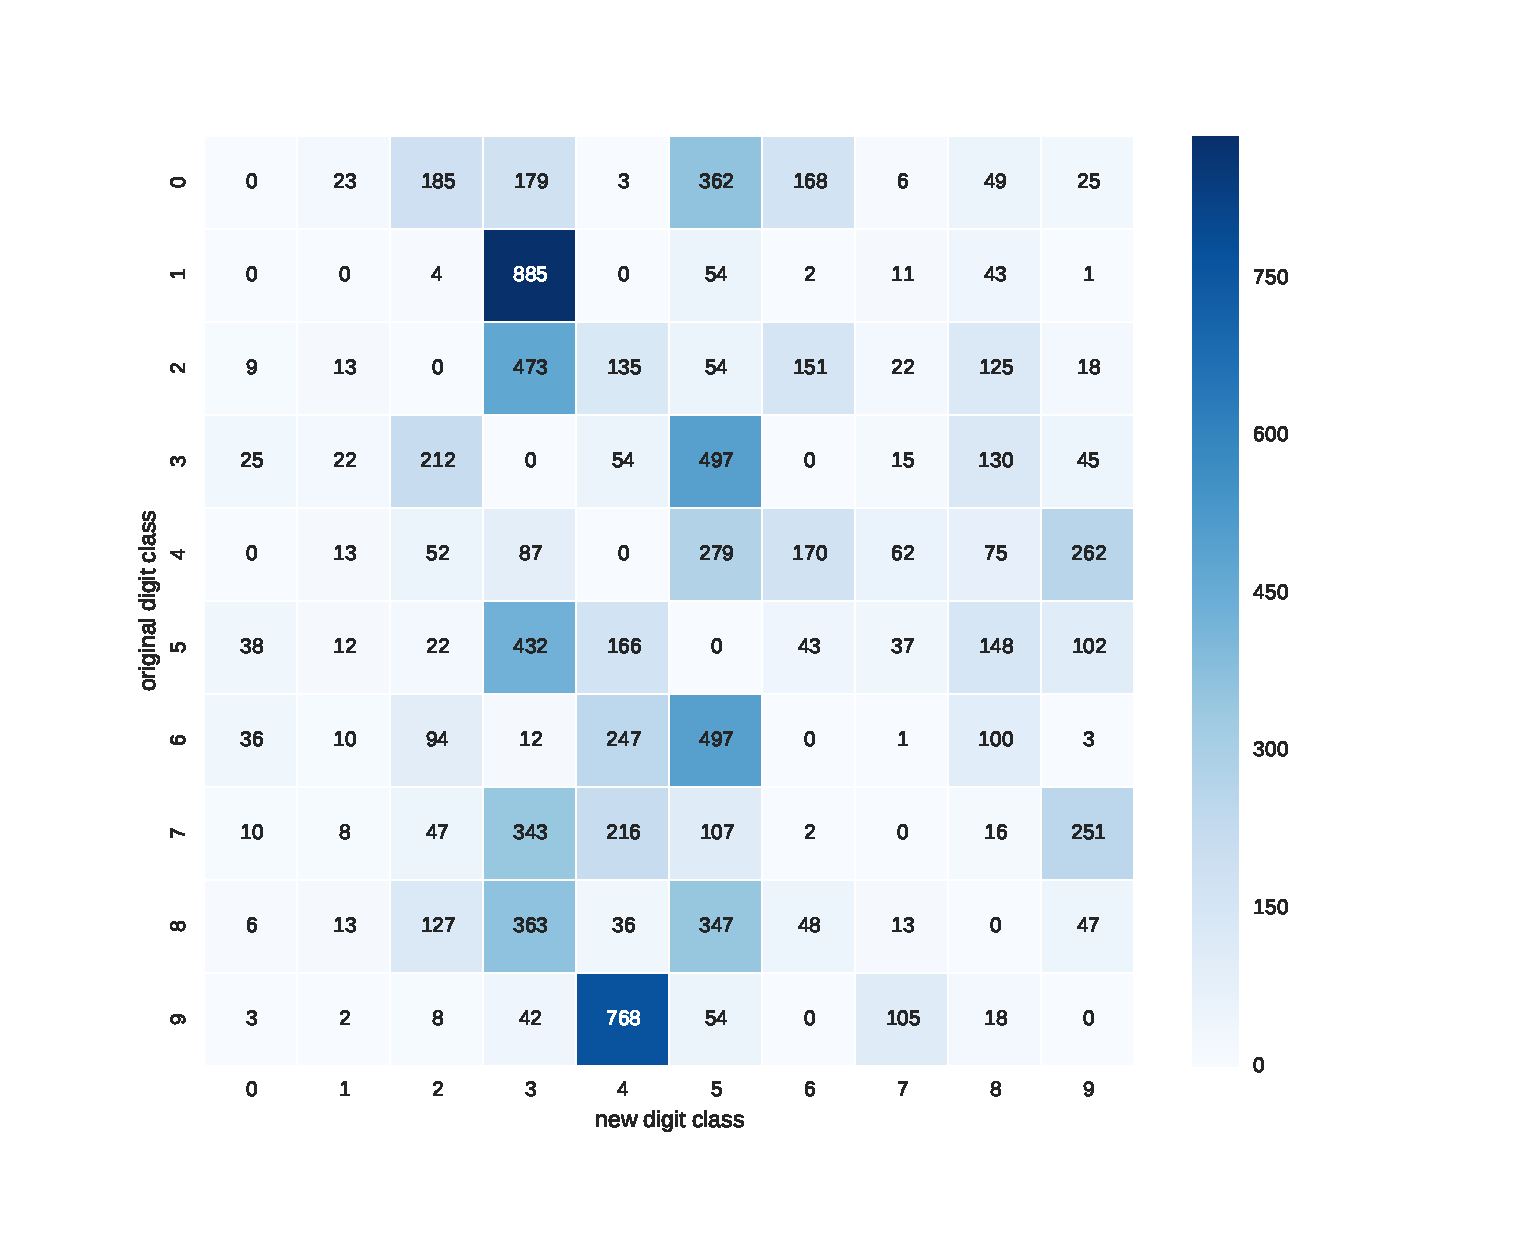
\includegraphics[scale=0.6]{figs/sup_3}
\label{exp:sup_3}
\caption{\small Classes of the adversarial examples generated.
For each original class, 1000 images were chosen (rows sum to 1000). We can see quite a strong bias to some classes, especially
for class 1 and 9.}
\end{center}
\end{figure}

\clearpage

\subsection{class-based distribution of squared euclidean norm}

\begin{figure}[h!]
\begin{center}
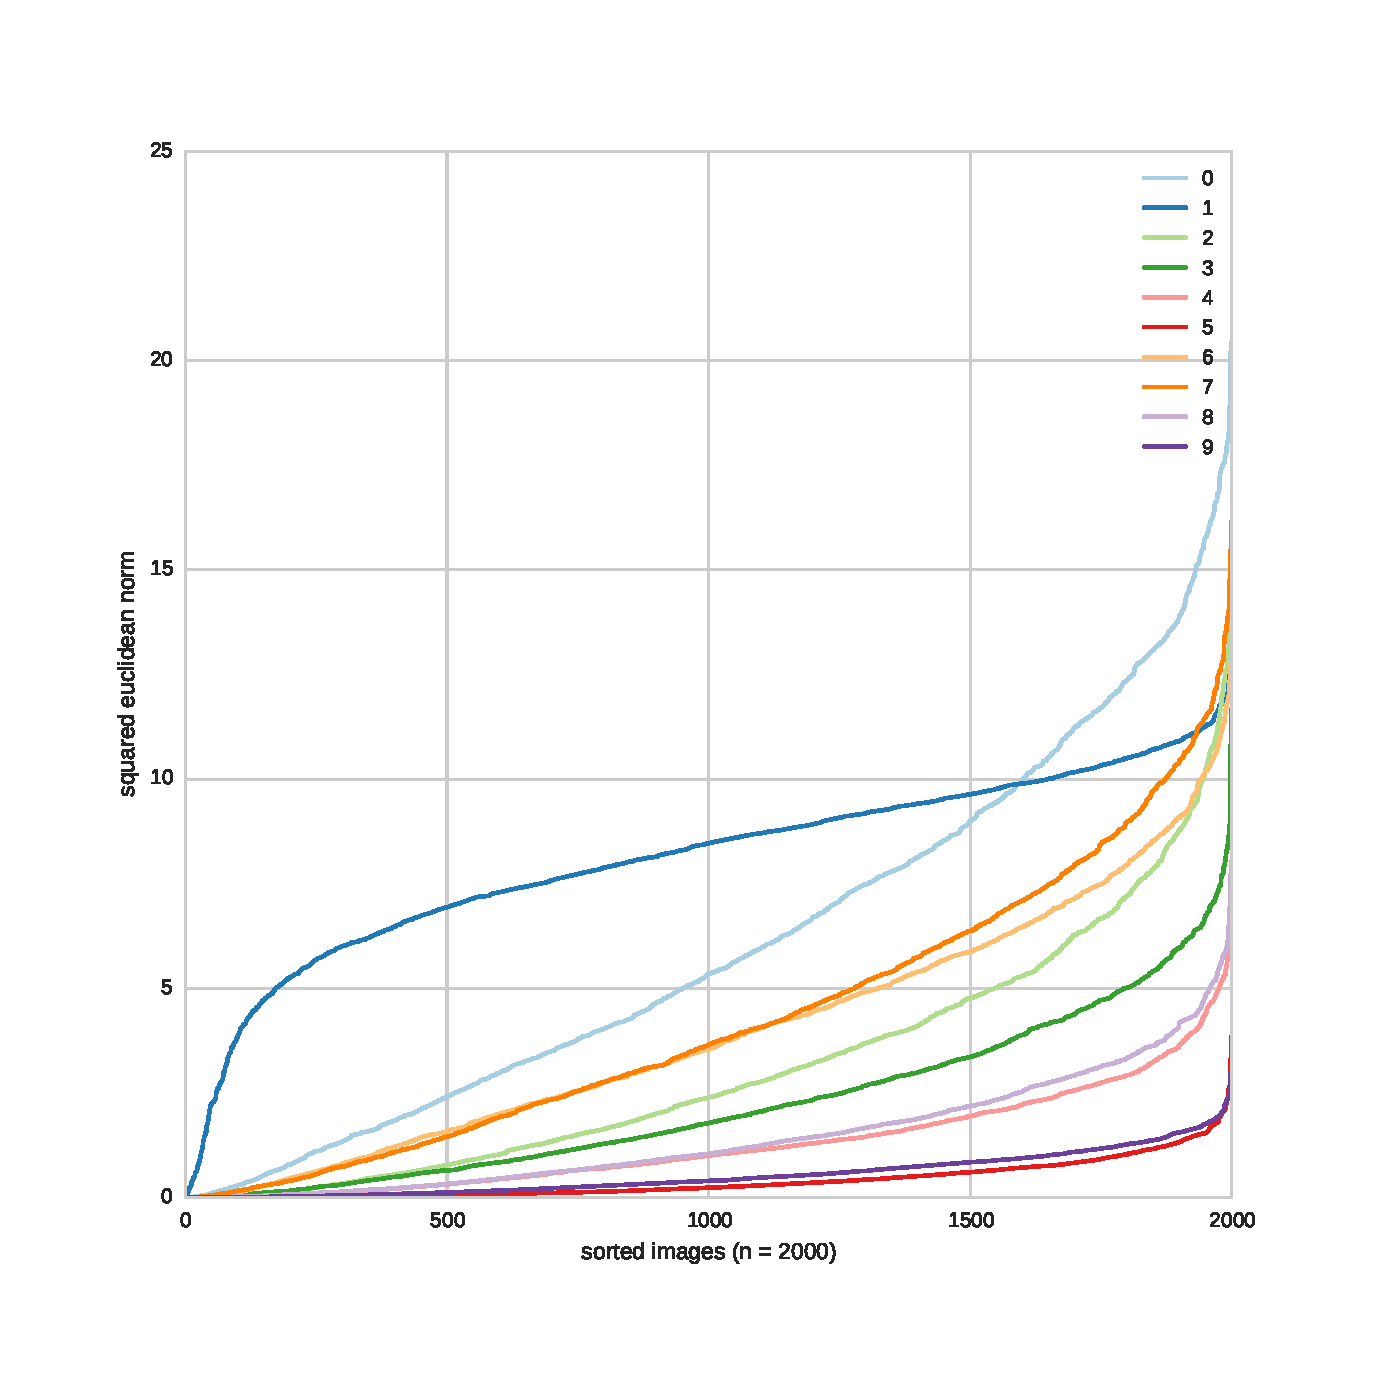
\includegraphics[scale=0.6]{figs/sup_4}
\label{exp:sup_4}
\caption{\small Comparison of the distribution of the squared norm for distorted images for each class of the
$\alpha=0.5$ $L^2$-regularized. Some classes are much
easier to generate adversarial examples from.}
\end{center}
\end{figure}

\null
\vfill
\raggedbottom
\pagebreak
\newpage


\subsection{example of input and adversarial images}

\begin{figure}[h!]
\begin{center}
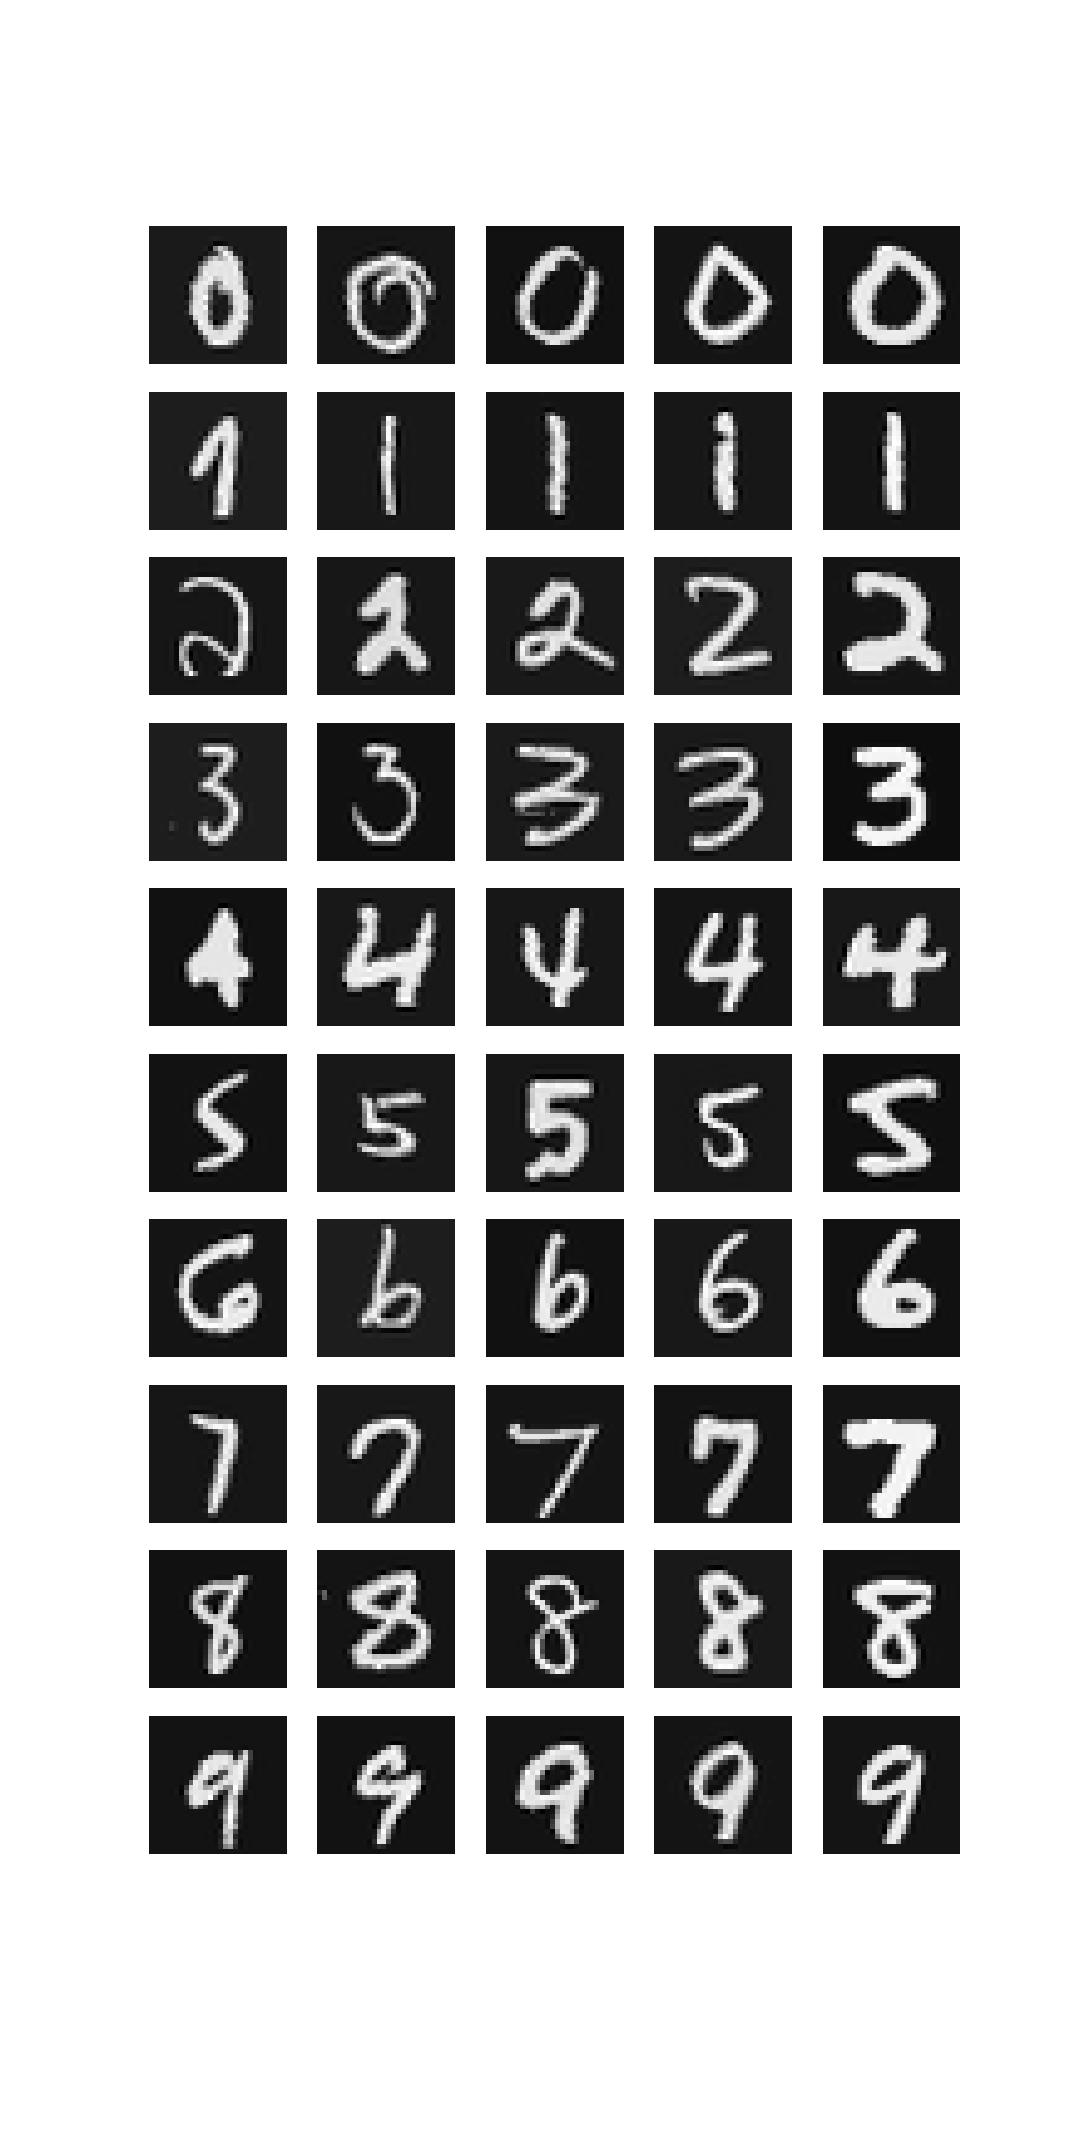
\includegraphics[scale=0.37]{figs/sup_5}
\label{exp:sup_5}
\caption{\small For each digit class, adversarial examples were generated. On each row, the 0, 50 and 100th percentiles of squared euclidean norms were chosen. The images are going from small to big from left to right. As can be observed, the smallest distortion is imperceptible but on the other hand, the median (50th percentile) is generally subtle. This is a good sign, meaning that the classifier is pretty robust.}
\end{center}
\end{figure}

\null
\vfill
\raggedbottom
\pagebreak
\newpage

\end{document}


